\documentclass[a4paper,twoside,11pt]{article}
\usepackage{a4wide,graphicx,fancyhdr,amsmath,amssymb,float,longtable}
\usepackage{algorithmic}
\usepackage{hyperref}
\usepackage{url}
\usepackage[superscript]{cite}
\usepackage{listings}
\usepackage[titletoc,toc]{appendix}
\usepackage{pdfpages}

%----------------------- Macros and Definitions --------------------------

\setlength\headheight{20pt}
\addtolength\topmargin{-10pt}
\addtolength\footskip{20pt}

\newcommand{\N}{\mathbb{N}}
\newcommand{\ch}{\mathcal{CH}}
\everymath{\displaystyle}
\newcommand{\solution}[1]{\noindent{\bf Solution to Exercise #1:}}

\fancypagestyle{plain}{%
\fancyhf{}
\fancyhead[LO,RE]{\sffamily\bfseries\large Technische universiteit Eindhoven}
\fancyhead[RO,LE]{\sffamily\bfseries\large 2IS55 Software Evolution}
\fancyfoot[LO,RE]{\sffamily\bfseries\large department of mathematics and computer science}
\fancyfoot[RO,LE]{\sffamily\bfseries\thepage}
\renewcommand{\headrulewidth}{0pt}
\renewcommand{\footrulewidth}{0pt}
}

\newcommand{\TODO}{{\color[rgb]{1,0,0} TODO}}
\newcommand{\av}{{\sc Azureus-Vuze}~}

\pagestyle{fancy}
\fancyhf{}
\fancyhead[RO,LE]{\sffamily\bfseries\large Technische universiteit Eindhoven}
\fancyhead[LO,RE]{\sffamily\bfseries\large 2IS55 Software Evolution}
\fancyfoot[LO,RE]{\sffamily\bfseries\large department of mathematics and computer science}
\fancyfoot[RO,LE]{\sffamily\bfseries\thepage}
\renewcommand{\headrulewidth}{1pt}
\renewcommand{\footrulewidth}{0pt}


\lstdefinestyle{customc}{
  belowcaptionskip=1\baselineskip,
  breaklines=true,
  frame=none,
  xleftmargin=\parindent,
  language=C,
  numbers=left,
  showstringspaces=false,
  basicstyle=\footnotesize\ttfamily,
  keywordstyle=\bfseries\color{green!40!black},
  commentstyle=\itshape\color{purple!40!black},
  identifierstyle=\color{blue},
  stringstyle=\color{orange},
  captionpos=b, 
}
\lstset{escapechar=@,style=customc}

%-------------------------------- Title ----------------------------------

\title{\sffamily\bfseries 2IS55 Software Evolution - Assignment 3}
\author{Mart Pluijmaekers \qquad Student number: 0753117 \\{\tt m.h.l.pluijmaekers@student.tue.nl}}

\date{\today}

%--------------------------------- Text ----------------------------------

\begin{document}
\maketitle
\tableofcontents
\newpage


\section{Introduction}
\label{sec:introduction}
In this paper we will be comparing many versions of \av against other versions in order to analyse the code duplication over these versions. We will be comparing 75 versions using the exact same process as Livieri et al.\cite{pap:liveiri} where the Linux kernel was analysed for code duplication. The tool our research used is called {\sc CCFinder}\cite{url:ccfinder} and was made available through a virtual machine also containing many versions of Azureus-Vuze. Using the information about duplication between all pairs we build a heat map, from which we will draw conclusions on the evolution of \av.


\section{Techniques used}
\label{sec:techniques}
In order to generate a heatmap visualizing the amount of code duplication between all pairs of versions of \av we have a few discrete steps. Firstly we want to detect all changes between all pairs, by doing some preparation work, do the actual comparison and lastly do some clean-up and parsing; all this is done through the tools provided by CCFinder. The second step consists of using Excel to generate a heatmap of the comparisons. \\

The workload was quite high and the computing power nowadays is quite high, therefore it lends itself well for a modular and multithreaded approach. We made scripts for each distinct step and set them up in such a way that we could divide the workload over multiple processors and so, speed up the computation process quite dramatically. \\

Since the multithreading support for CCFinder is lacking, we decided to do the multithreading ourselves using our scripts. Firstly we started by making multiple copies of the source code. Making sure that we have a unique copy available for each script executing part of the workload makes sure that they do not interfere when working on the source files. Since the comparison of versions is symmetric, we do not need to check version $A$ to $B$ and version $B$ to $A$. This unfortunately means that we cannot trivially divide up the workload but need to do some computations. Since the fourth version needs to be compared to $n-4-1$ versions, while the second to last version only needs to be compared to a single other version. \\

We solved this problem by checking the amount of work needed and divide it by the number of desired compute threads. Then through an iterative process we determine the start and end for each compute thread and start them. Since after preprocessing we are left with a list of files we are now able to easily split the work. All the scripts except one have been written in {\sc PHP}\cite{url:php}, the single script written in . \\

Since there were some minor issues with an invisible character in a file called {\sc FileHandler.java} which is contained in many versions of \av we simply opened all of them and saved them using a simple text editor in order to remedy this issue. \\

There are five scripts in total, only a single one of these is used to do an automated devision of labour, since the other cases are more trivial. These are listed in Appendix \ref{app:scripts}. The workings of the computation scripts are listed below and are grouped to the .

\subsection{Precompute}

\subsection{Code duplication detection}

\subsection{Cleanup \& parsing}


\section{CCFinder discussion}
\label{sec:ccfinderdiscussion}
CCFinder is token based clone detection a tool proposed by Kamiya et al.\cite{pap:ccfinder} in 2001 and is used for detecting code duplication between different pieces of software. We specifically use it for detecting code duplication between distinct versions of the same tool. 


\subsection{Clone detection}
\label{sec:cloneDetection}
CCFinder can detect many but not all clone-types; each type is listed below and discussed.

\subsubsection{Type 1 clones}
\label{sec:type1}
Type 1 clones are exact copies, which can be detected by CCFinder since it can also detect type 2 clones.

\subsubsection{Type 2 clones}
\label{sec:type2}
CCFinder transforms all identifiers to some specific token making sure that it can detect type 2 clones since it can now check the tokens which can be completely separate from the names of the identifiers.

\subsubsection{Type 3 clones}
\label{sec:type3}
Type 3 clones are clones where the code is similar but some statements have been added, removed or changed. The unchanged parts can naturally be detected as gapped clones. CCFinder can detect these clones when a threshold value is given and taken into account for the gaps between the parts.

\subsubsection{Type 4 clones}
\label{sec:type4}
When two pieces of software implement the same concepts but in a different manner we call it a type 4 clone. CCFinder unfortunately cannot detect these clones since it is a token based tool and therefore cannot detect type 4 clones.


\section{Azureus-Vuze discussion}
\label{sec:azureusdiscussion}
{\sc Azureus} is a project which started in June of 2003 (released in July) as a general purpose BitTorrent client. Not only can it be used for downloading torrent files; but also for uploading original video content. Over the years Azureus grew to one of the major torrent clients, but rebranded itself to {\sc Vuze} in 2006 because it wanted to be a social platform too. At first a seperate Azureus version was available too, but from June 2008 onwards the developers stopped releasing pure Azureus versions of the software.  \\

The current stable version of {\sc Vuze} is 5.6.0.0 (March 3$^{\text{rd}}$ 2015) containing a total of 941.461 lines of (Java) code for a total size of 42MB. While the oldest version available to us (2.0.0.8) has 68.664 lines of (Java) code for a total size of 1.4MB. \\

We set the goal to analyse all 79 versions of {\sc Azureus-Vuze} available to us, but due to a mistake of the scheduling script, we only managed 75 versions unfortunately we did not have enough time after the detection to compute the required values for the remaining four versions. The versions that were tested are: \\

\begin{tabular}{cccccccccccc}
2008 & 2010 & 2025 & 2026 & 2027 & 2030 & 2032 & 2040 & 2042 & 2060 & 2070 & 2080 \\
2082 & 2084 & 2100 & 2102 & 2104 & 2200 & 2202 & 2300 & 2302 & 2304 & 2306 & 2400 \\
2402 & 2500 & 2502 & 2504 & 3006 & 3008 & 3010 & 3012 & 3014 & 3016 & 3020 & 3022 \\
3030 & 3034 & 3040 & 3042 & 3050 & 3052 & 3100 & 3110 & 4000 & 4002 & 4004 & 4100 \\
4102 & 4104 & 4200 & 4202 & 4204 & 4208 & 4300 & 4302 & 4304 & 4306 & 4310 & 4312 \\
4314 & 4400 & 4402 & 4404 & 4406 & 4410 & 4500 & 4502 & 4504 & 4510 & 4600 & 4602 \\
4604 & 4700 & 4710 &      &      &      &      &      &      &      &      &      \\
\end{tabular}


\section{Heat map}
\label{sec:heatmap}
The generated heatmap can be seen in figure \ref{fig:heatmap}. Green indicates low code duplication while red indicates high code duplication. \\

As we can see the code duplication increases as the version increases since the code keeps growing and old (reliable/correct) code does not change any more. Furthermore we can clearly see that between 2 sequential versions the code duplication is high, which makes sense since the differences between these versions should be small.
\begin{figure}[!h]
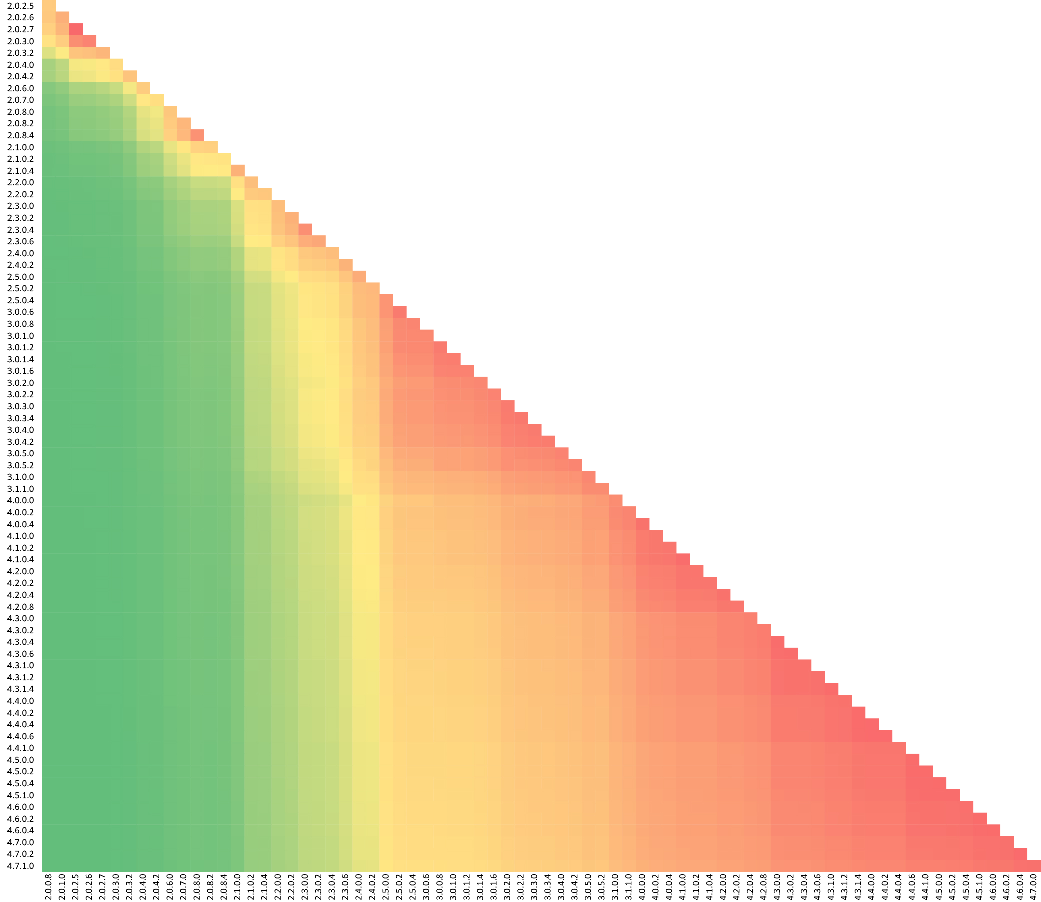
\includegraphics[scale=0.8]{../results/heatMap.pdf}
\caption{The heatmap of all checked versions of \av}
\label{fig:heatmap}
\end{figure}

\section{Discussion of evulution}
\label{sec:discussion}
Lorem ipsum dolor sit amet, consectetur adipiscing elit. Aenean vel enim in felis vehicula rutrum dictum sodales nibh. Pellentesque tempor metus nibh, eu gravida tellus auctor eu. Nunc et lorem sem. Suspendisse dui risus, fringilla ut ante a, pretium pretium dolor. Vivamus non ipsum a justo laoreet rutrum ut eu ipsum. Nulla tempor sed metus ornare faucibus. Pellentesque tincidunt interdum viverra.

Interdum et malesuada fames ac ante ipsum primis in faucibus. Duis tellus libero, blandit quis volutpat et, rutrum molestie lectus. Cras vitae consequat sem. Nullam sit amet urna ac diam accumsan accumsan sed vel risus. Cras sem ante, mattis id erat vel, auctor finibus ante. Proin posuere massa auctor nulla rhoncus laoreet. Praesent egestas placerat accumsan. Pellentesque pellentesque orci massa. Fusce eu tristique justo, a ornare est. Integer eget metus metus. Aliquam quis sem id eros facilisis fermentum. Suspendisse malesuada sodales orci tristique tincidunt. Vestibulum ac nulla quis augue venenatis volutpat et in turpis.

Morbi porttitor interdum purus a pellentesque. Proin placerat libero vitae nunc lacinia, nec consectetur arcu egestas. Fusce porta bibendum pretium. Donec et sodales tellus. Nunc ut consequat nulla. Fusce nisi augue, aliquet id hendrerit cursus, semper at orci. Phasellus ac imperdiet ante, non faucibus mauris.

Duis aliquet libero a lacinia feugiat. Vivamus blandit urna id neque sollicitudin posuere. Maecenas tempor non ex non fermentum. Nullam nec congue turpis. Etiam tincidunt massa ut libero dignissim vulputate. Aenean rhoncus ligula urna, vel suscipit erat fringilla non. Phasellus dapibus orci massa, suscipit porta lorem iaculis vitae. Nulla quis turpis eu dui interdum elementum non et lorem.

Etiam luctus sit amet diam a iaculis. Nulla luctus nunc id lorem cursus, fermentum euismod orci luctus. Curabitur et eleifend est. Aliquam eu risus facilisis felis lacinia porttitor eget ac dui. Suspendisse eleifend ultrices lacus, eget ornare risus laoreet et. Ut nibh mauris, rhoncus sed lobortis at, interdum ut nulla. In accumsan, ligula vitae porttitor congue, ante diam dictum nisi, eget mattis lacus metus eget ex. Praesent id tortor purus. Praesent commodo lorem ipsum, ut sodales ipsum mattis ut. Morbi sed cursus sem.


\begin{thebibliography}{9}
\bibitem{pap:liveiri}
Simone Livieri, Yoshiki Higo, Makoto Matsushita, and Katsuro Inoue. ``Analysis of the Linux Kernel Evolution Using Code Clone Coverage'' Proceedings of the Fourth International Workshop on Mining Software Repositories,  pp. 22-1 22-4, Washington, DC, USA, 2007.

\bibitem{pap:ccfinder}
Toshihiro Kamiya, Fumiaki Ohata, Kazuhiro Kondou, Shinji Kusumoto, and Katuro Inoue: "Maintenance support tools for Java programs: CCFinder and JAAT", Proc. of The 23rd Int'l Conf. on Software Eng, pp. 837-838, Toronto, Canada, (May, 2001).

\bibitem{url:php}
Zend. PHP - PHP: Hypertext Preprocessor. Available: \url{http://php.net/}
\bibitem{url:ccfinder}
Toshihiro Kamiya. CCFinder a code-clone detector. Available: \url{http://www.ccfinder.net/}

\end{thebibliography}

\newpage

\begin{appendices}
\section{Scripts}
\label{app:scripts}


\lstinputlisting[language=Php,caption={devideThing.php - Devides up the workload over multiple instances of {\sc exec.php}},label={lst:devideThing}]{../code/devideThing.php}

\newpage

\lstinputlisting[language=Php,caption={exec.php - Precompute source folders to make analysis possible},label={lst:exec}]{../code/exec.php}

\newpage

\lstinputlisting[language=Php,caption={analyze.php - Executes an analysis over the precomputed files for a subset of the computed version pairs.},label={lst:analyze}]{../code/analyze.php}

\newpage

\lstinputlisting[language=Php,caption={calculate.php - Executes the actual analysis of a subset of version pairs},label={lst:calculate}]{../code/calculate.php}



\lstinputlisting[language=bash,caption={calcLoc.sh - Calculates and stores the total lines of code for each version},label={lst:calcloc}]{../code/calcLoc.sh}

\newpage

\lstinputlisting[language=bash,caption={parse.php - Parse the files generated by {\sc calculate.php} to make them formatted for easy heatmap generation},label={lst:parse}]{../code/parse.php}

\end{appendices}


\end{document}
